This section introduces basic \LaTeX\ syntax. Learn how to configure the project Preamble then write your first section in \LaTeX\ code!
\subsection{Basic LaTeX}
Authoring with \LaTeX\ is similar to writing a program: type code to define program behavior, compile program into consumable file, then open file and enjoy! There are four key principles to consider when authoring documents with \LaTeX:
\begin{enumerate}
    \item Content is written in plaintext.
    \item Formatting and features are applied with commands.
    \item Packages provide extra text, graphics, and presentation commands.
    \item \LaTeX\ code is typically compiled into a read-only professional-looking PDF.
\end{enumerate}
With these principles in mind, let's start learning some basic \LaTeX\ syntax and commands\footnote{Based on existing instructional material: http://www.rpi.edu/dept/arc/training/latex/class-slides-pc.pdf}.
%TODO: Cite this
\par
The \verb|"\"| backslash character is used to begin all \LaTeX\ commands. E.g.
\verb|\LaTeX| compiles to \LaTeX.
\par
Some commands take input enclosed in curly braces. E.g.\\
\verb|\textit{This text is italicized}| $\rightarrow$ \textit{This text is italicized}.
\par
{\large\textbf{Common commands include:}}\\
\verb|\\|, \verb|\newline|, \verb|\par|\\
Various ways to generate new lines.
\par
\verb|\newpage|\\
Insert page break to start text on new page.
\par
\verb|\textit{text}|, \verb|\textbf{text}|, \verb|\texttt{text}|\\
Modifies text to be \textit{italicized}, \textbf{bold}, or \texttt{scientific}.
\par
\verb|\usepackage{<packageName>}|\\
Define a \LaTeX\ package to use for modular commands and behaviors in your project.
\par
\verb|\chapter{<title>}|, \verb|\section{<title>}|, \verb|\subsection{<title>}|\\
Mark the beginning of new chapters/sections/subsections.
\par
\verb|\title{<document title>}|, \verb|\author{<author>}|, \verb|\date{<date>}|\\
Define the document's title, author, and date.
\par
\verb|\maketitle|\\
Print the document's title, author, and date.
\par
\verb|\markboth{left title}{right title}|\\
Defines the headings or footings on either side of the page.
\par
\verb|\url{<website link>}|\\
Prints a clickable website link on the page.
\par
\verb|\today|\\
Print today's date.
\par
{\large\textbf{Certain characters have special meanings in \LaTeX.}}\\
\begin{tabular}{r|l}
\textbf{Char} & \textbf{Meaning} \\
\verb|%|& Parameter in a macro; also used in tables \\ 
\verb|$|& Used to begin and end math mode \\
\verb|%|& Used for comments in the source file \\
\verb|&|& Tab mark, used in alignments and tables \\
\end{tabular}
\par

{\large\textbf{Environments are uniquely formatted blocks of text}}\\
Environments define blocks of texts that receive special formatting or processing. They are delimited by the \verb|\begin{<type>}| and \verb|\end{<type>}| commands that take . Everything between \verb|\begin| and \verb|\end| will be processed based on the environment <type> inputted.
\par
For now, you only need knowledge about the \texttt{document} and \texttt{abstract} environment types:\\
\begin{itemize}
\item\verb|\begin{document}| and \verb|\end{document}|\\
Define area for all document text. Everything included inside the \verb|begin{document}| \verb|\end{document}| commands will be rendered in the final document.

\item\verb|\begin{abstract}| and \verb|\end{abstract}|\\
Define area for the abstract of the document. The abstract is uniquely formatted by the template to give readers a quick summary about the document.

\item\verb|\begin{minipage}{<width>}| and \verb|\end{minipage}|\\
Define area for minipage. Minipages are useful for containing graphics and other contents in a single paragraph box.
\end{itemize}

\par
To learn more about environments, see Overleaf's tutorial at \url{https://www.overleaf.com/learn/latex/Environments}.\\
For a comprehensive guide about \LaTeX\ syntax and commands, see \url{https://www.rpi.edu/dept/arc/docs/latex/latex-intro.pdf}.\\
To learn more about \LaTeX\ document structure, see \url{https://www.overleaf.com/learn/latex/Creating_a_document_in_LaTeX}.
\par
In the next subsection, you will use basic knowledge of \LaTeX\ to configure the \texttt{preamble} of your project.

\subsection{Preamble and Abstract}
We previously set the \texttt{Main Document} of the project in Overleaf to
\path{layout_e.tex}. Locate this file and open it to begin editing the \texttt{preamble}.

\begin{minipage}{\linewidth}
\centering
\fbox{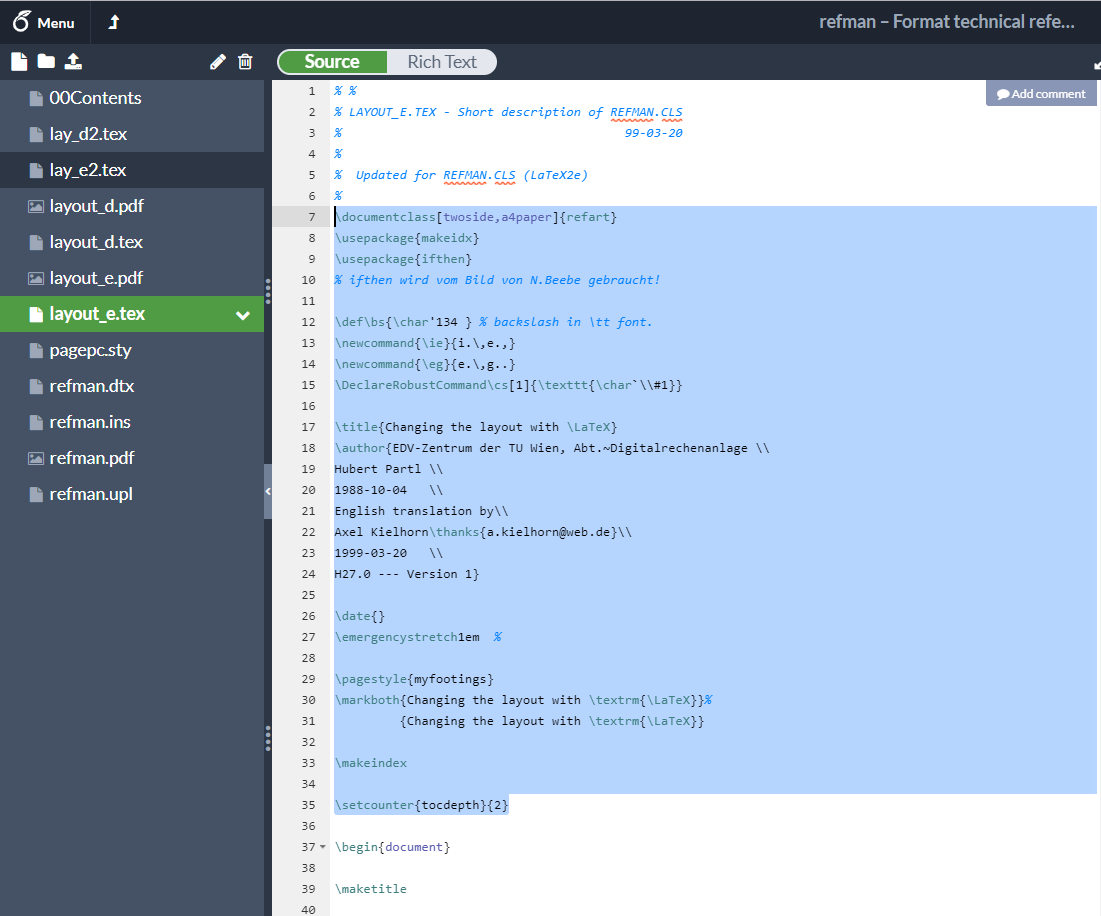
\includegraphics[width=\linewidth]{graphics/MainDocumentPreamble.PNG}}
\captionof{figure}{Locating \detokenize{layout_e.tex file}}
\label{fig:Preamble}
\end{minipage}

Notice the highlighted section in figure \ref{fig:Preamble}. The area of from the start of the document to the \verb|\begin{document}| command is called the \texttt{preamble}: the first part the main document where you describe the title, packages used, and more information about the document. Configuring the \texttt{preamble} is necessary to customize the \LaTeX\ project for your project's requirements.

    \subsubsection{Adding Packages}
First, extend the available commands in your \LaTeX\ project. Locate the \verb|\usepackage{ifthen}| command around \texttt{line 9}. Copy-paste the following commands after that line to start writing with several useful packages:
\par
\begin{minipage}{\linewidth}
\begin{verbatim}
\usepackage{url} %Clickable URLs
\usepackage{csquotes} %Advanced quotations
\usepackage{graphicx} %Add graphics
\usepackage{caption} %Captioning for figures
\usepackage{xcolor} %Change text color
\usepackage{nameref} %Reference labels by name
\usepackage{titlesec} %Modify sectioning behavior
\usepackage[T1]{fontenc} %Change font encoding
\usepackage{verbatim} %Print text verbatim
\end{verbatim}
\end{minipage}
\par
We will explore some commands in these packages in the later \nameref{sec:Extended Writing} section.\\

    \subsubsection{Title, Author, and Date}
Configure the heading information of the document by modifying input in the \verb|\title|, \verb|\author|, and \verb|\date| commands. For example, locate the \verb|\title| command and customize the input to whatever you want:
\par
\textbf{Original:}\\
\verb|\title{Changing the layout with \LaTeX}|
\par
\textbf{Modified:}\\
\verb|\title{Overleaf Guide Guide :D}|
\par
Similarly, configure the \texttt{author} and \texttt{date} of the document by change the text inside the curly brackets. Use \verb|\\| for creating new lines in text.
\par
\begin{minipage}{\linewidth}
\begin{verbatim}
\author{
    John Pan (jpthek9@gmail.com)\\
    \url{https://github.com/SnpM}\\
    John likes Ed Sheeran.
}
\end{verbatim}
\end{minipage}
\par
...
\par
\begin{minipage}{\linewidth}
\begin{verbatim}
\date{
    \url{https://github.com/SnpM/latex-guide-guide.git}\\
    \today\\
    Today is National Pet Day.
}
\end{verbatim}
\end{minipage}
\par



    
\subsection{Adding Content}
   Now that the preamble is set up and you're more familiar with \LaTeX\, it's time to begin writing content for the document. This subsection details how to modify the \textit{Abstract} and individual sections of the document.
    
    \subsubsection{Modifying Abstract}    
    The \textit{abstract} of the document is one of the first parts of the document environment; it is a block of text specially formatted for delivery of the document's purpose to readers. The abstract is defined within the \verb|begin{abstract}| and \verb|\end{abstract}| \textit{environment}. To modify the document's abstract, locate and edit the text after the \verb|\begin{abstract}| command. Try to experiment with different font faces and other \LaTeX\ commands such as \verb|\url{<website link>}|.
    
    \begin{minipage}{\linewidth}
        \centering
        \fbox{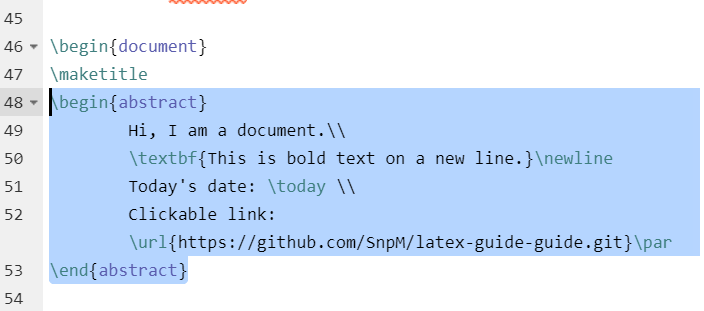
\includegraphics[width=.95\linewidth]{graphics/Abstract.PNG}}
        \captionof{figure}{Source for customized abstract}
        \label{fig:Preamble}
    \end{minipage}
 
    \subsection{Modifying Sections}
    Sections are different from the \textit{abstract} because they are not defined with environments (\verb|\begin ... \end|). Instead, sections are defined with a single command indicating the start of the section. The section automatically continues until another section is defined or the document ends.
    \par
    Navigate to the first section identified by the first \verb|\section| command.
    \begin{minipage}{\linewidth}
        \centering
        \fbox{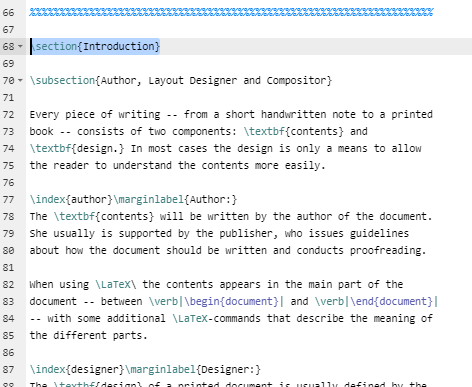
\includegraphics[width=.95\linewidth]{graphics/FirstSection.PNG}}
        \captionof{figure}{The first section is titled \textit{Introduction}}
        \label{fig:Preamble}
    \end{minipage}
    
    